\section{Two nodes together}

\begin{figure}[htbp]
    \centering
    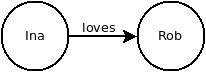
\includegraphics[width=120mm]{./P1.start/01_node-to-node.jpeg}
    \caption{A simple link}
    \label{odb2Nodes}
\end{figure}


\begin{lstlisting}
; 2nodes.cpp

#include <iostream>

#include "generic.h"
#include "odb.h"

auto oOdb = odb::COdb();

int main()
    {
    // 2 people
    oOdb.MakeNode("Ina");
    oOdb.MakeNode("Rob");
    
    // a relation
    oOdb.MakeReason("loves");
    
    // binding
    oOdb.LinkNode2Node("Ina", "loves", "Rob");
    
    // show us
    std::cout << "---------------- all nodes" << '\n';
    for ( auto const & a:oOdb.Nodes() )
        {
        std::cout << *a << '\n';
        }
    }
\end{lstlisting}

Beschreibender Text

\begin{itemize}
\item  create nodes
\item  create reason
\item  link node with reason
\end{itemize}


